\documentclass[aspectratio=169,10pt]{beamer}

% ==============================================================================
% CẤU HÌNH NGÔN NGỮ & FONT CHỮ TIẾNG VIỆT
% ==============================================================================
\usepackage[utf8]{inputenc}
\usepackage[vietnamese]{babel}
\usepackage[T5]{fontenc}
\usepackage{lmodern}

% Cấu hình ký tự unicode đặc biệt
\DeclareUnicodeCharacter{251C}{|--}
\DeclareUnicodeCharacter{2500}{-}
\DeclareUnicodeCharacter{2514}{\`--}
\DeclareUnicodeCharacter{2502}{|}
\DeclareUnicodeCharacter{2014}{--}

% ==============================================================================
% GIAO DIỆN CHỦ ĐỀ & MÀU SẮC CÔNG NGHỆ CAO (CYBER TECH / DEVOPS THEME)
% ==============================================================================
\usetheme{Madrid}
\usecolortheme{whale}

% Định nghĩa bảng màu công nghệ
\definecolor{techbg}{RGB}{11, 15, 25}        % Nền xanh đen sâu
\definecolor{techprimary}{RGB}{14, 116, 144}  % Cyan/Teal đậm
\definecolor{techaccent}{RGB}{56, 189, 248}   % Sky Blue sáng
\definecolor{techdark}{RGB}{15, 23, 42}       % Slate Dark
\definecolor{techemerald}{RGB}{16, 185, 129}  % Xanh lá thành công
\definecolor{techpurple}{RGB}{168, 85, 247}   % Tím công nghệ
\definecolor{techamber}{RGB}{245, 158, 11}    % Vàng cảnh báo

% Áp dụng màu sắc vào Beamer
\setbeamercolor{palette primary}{bg=techprimary,fg=white}
\setbeamercolor{palette secondary}{bg=techdark,fg=white}
\setbeamercolor{palette tertiary}{bg=techbg,fg=white}
\setbeamercolor{titlelike}{parent=palette primary,fg=techaccent,bg=techdark}
\setbeamercolor{frametitle}{bg=techdark,fg=techaccent}
\setbeamercolor{block title}{bg=techprimary,fg=white}
\setbeamercolor{block body}{bg=techdark!10,fg=black}
\setbeamercolor{block title example}{bg=techemerald,fg=white}
\setbeamercolor{block body example}{bg=techemerald!10,fg=black}
\setbeamercolor{block title alerted}{bg=techamber,fg=white}
\setbeamercolor{block body alerted}{bg=techamber!10,fg=black}

\setbeamertemplate{navigation symbols}{} % Ẩn thanh điều hướng mặc định
\setbeamertemplate{footline}[frame number]

% ==============================================================================
% GÓI HỖ TRỢ ĐỒ HỌA & BẢNG BIỂU
% ==============================================================================
\usepackage{graphicx}
\usepackage{booktabs}
\usepackage{listings}
\usepackage{tikz}
\graphicspath{{images/}{./}{../docs/images/}}

\lstset{
    basicstyle=\ttfamily\scriptsize,
    backgroundcolor=\color{techdark!8},
    frame=single,
    rulecolor=\color{techprimary!40},
    keywordstyle=\color{techprimary}\bfseries,
    stringstyle=\color{techemerald},
    commentstyle=\color{gray}\itshape,
    breaklines=true,
    showstringspaces=false
}

% ==============================================================================
% THÔNG TIN BÁO CÁO ĐỀ TÀI
% ==============================================================================
\title[Đồ Án: QL Kho Hàng \& DevOps]{XÂY DỰNG VÀ TRIỂN KHAI\\HỆ THỐNG QUẢN LÝ KHO HÀNG THÔNG MINH}
\subtitle{Kiến Trúc Đa Tầng Container, Gateway SSL, Giám Sát Prometheus \& Phân Tích Log Loki}
\author[Thân Phú Cường]{
    \textbf{Sinh viên thực hiện:} Thân Phú Cường -- DTC245200356 (Lớp CNTTK23L)\\[2pt]
    \textbf{Giảng viên hướng dẫn:} TS. Vũ Văn Diện
}
\institute[ICTU]{
    Học phần: Triển khai \& Quản trị Hệ thống / DevOps\\
    Trường Đại học Công nghệ Thông tin và Truyền thông -- Đại học Thái Nguyên
}
\date{Năm học 2025 -- 2026}

\begin{document}

% ------------------------------------------------------------------------------
% FRAME 1: TRANG TIÊU ĐỀ
% ------------------------------------------------------------------------------
\begin{frame}
    \titlepage
\end{frame}

% ------------------------------------------------------------------------------
% FRAME 2: ĐẶT VẤN ĐỀ & MỤC TIÊU
% ------------------------------------------------------------------------------
\begin{frame}{1. Đặt Vấn Đề \& Mục Tiêu Kỹ Thuật Đề Tài}
    \begin{columns}[T]
        \begin{column}{0.48\textwidth}
            \begin{block}{Thách Thức Kho Hàng Truyền Thống}
                \begin{itemize}
                    \item Sai lệch tồn kho do nhập liệu thủ công bằng bảng tính Excel.
                    \item Chậm trễ cập nhật hàng cạn kiệt (\textit{Low-stock}).
                    \item Hạ tầng đơn khối, thiếu an toàn thông tin.
                    \item Thiếu cơ chế giám sát sức khỏe và phân tích lỗi tập trung.
                \end{itemize}
            \end{block}
        \end{column}
        
        \begin{column}{0.48\textwidth}
            \begin{exampleblock}{5 Trụ Cột Vận Hành DevOps Đạt Được}
                \begin{enumerate}
                    \item \textbf{Containerization:} Cụm 10 dịch vụ Docker Compose.
                    \item \textbf{Gateway SSL:} Nginx Reverse Proxy \& 5 Security Headers.
                    \item \textbf{Monitoring:} Prometheus (15s Pull) \& Grafana Dashboard.
                    \item \textbf{Logging:} Loki, Promtail \& 3 truy vấn LogQL chuẩn.
                    \item \textbf{Hardening:} Non-root user, 3 subnet mạng cô lập.
                \end{enumerate}
            \end{exampleblock}
        \end{column}
    \end{columns}
\end{frame}

% ------------------------------------------------------------------------------
% FRAME 3: KIẾN TRÚC TỔNG THỂ 4 TẦNG
% ------------------------------------------------------------------------------
\begin{frame}{2. Kiến Trúc Hạ Tầng 4 Tầng Toàn Diện (Multi-Tier Architecture)}
    \begin{center}
        \begin{tabular}{|p{0.18\textwidth}|p{0.75\textwidth}|}
            \hline
            \textbf{Tầng 1: Client} & Trình duyệt Web (Chrome, Edge, Firefox) gửi yêu cầu HTTPS:443 mã hóa TLS. \\
            \hline
            \textbf{Tầng 2: Gateway} & \textbf{Nginx Reverse Proxy}: Điểm chạm duy nhất, chuyển hướng 301 HTTP $\to$ HTTPS, giải mã SSL RSA 2048-bit, 5 Security Headers. \\
            \hline
            \textbf{Tầng 3: App \& DB} & \textbf{Web Kho (PHP 8.2)} + \textbf{MySQL 8.0} + \textbf{phpMyAdmin}. Cơ sở dữ liệu nằm trong subnet cô lập \texttt{backend-net}, không mở cổng 3306 ra ngoài. \\
            \hline
            \textbf{Tầng 4: SRE \& Logs} & \textbf{Prometheus} (scrape 15s) + \textbf{Grafana} (Dashboard trực quan) + \textbf{Loki} (Kho log tối ưu) + \textbf{Promtail} (Thu thập log Nginx/App) + \textbf{Exporters}. \\
            \hline
        \end{tabular}
    \end{center}
    \vspace{4pt}
    \begin{exampleblock}{Đặc Điểm Vận Hành}
        Phân tách 3 mạng Docker bridge: \texttt{frontend-net}, \texttt{backend-net}, \texttt{monitoring-net}. Triệt tiêu nguy cơ tấn công xâm nhập ngang (Lateral Movement).
    \end{exampleblock}
\end{frame}

% ------------------------------------------------------------------------------
% FRAME 4: CỤM DOCKER & GIT WORKFLOW
% ------------------------------------------------------------------------------
\begin{frame}{3. Quản Trị Cụm 10 Services \& Git Milestone Workflow}
    \begin{columns}[T]
        \begin{column}{0.48\textwidth}
            \begin{block}{Cụm 10 Services (Docker Compose)}
                \begin{itemize}
                    \item \texttt{nginx-gateway}: Reverse Proxy \& SSL
                    \item \texttt{web-inventory-app}: Ứng dụng Web PHP 8.2
                    \item \texttt{mysql-db}: Cơ sở dữ liệu MySQL 8.0
                    \item \texttt{phpmyadmin}: Quản trị CSDL qua \texttt{/pma/}
                    \item \texttt{prometheus}: Máy chủ lưu trữ Time-series
                    \item \texttt{grafana}: Trực quan hóa Dashboard
                    \item \texttt{loki} \& \texttt{promtail}: Thu thập \& nén Logs
                    \item \texttt{mysql\_exporter} \& \texttt{node\_exporter}
                \end{itemize}
            \end{block}
        \end{column}

        \begin{column}{0.48\textwidth}
            \begin{exampleblock}{Git Workflow 3 Commit Chuẩn Mực}
                \begin{itemize}
                    \item \textbf{Commit 1 (Yêu cầu 3):} Cấu hình Nginx Gateway, chuyển hướng HTTPS 301, chứng chỉ SSL và 5 Security Headers.
                    \item \textbf{Commit 2 (Yêu cầu 4):} Triển khai hệ thống giám sát Prometheus, thiết lập Exporters và tự động nạp Grafana Dashboard.
                    \item \textbf{Commit 3 (Yêu cầu 5):} Triển khai quản lý log tập trung với Grafana Loki, Promtail và 3 truy vấn LogQL chuyên sâu.
                \end{itemize}
            \end{exampleblock}
        \end{column}
    \end{columns}
\end{frame}

% ------------------------------------------------------------------------------
% FRAME 5: THIẾT KẾ CSDL MYSQL 8.0
% ------------------------------------------------------------------------------
\begin{frame}[fragile]{4. Thiết Kế Cơ Sở Dữ Liệu MySQL 8.0 \& Toàn Vẹn ACID}
    \begin{columns}[T]
        \begin{column}{0.5\textwidth}
            \begin{block}{6 Bảng Dữ Liệu Chuẩn Hóa 3NF}
                \begin{itemize}
                    \item \texttt{users}: Phân quyền RBAC (\texttt{admin}/\texttt{staff}), mật khẩu BCRYPT, session HttpOnly.
                    \item \texttt{categories}: Phân nhóm danh mục sản phẩm.
                    \item \texttt{products}: SKU, giá nhập, giá bán, tồn kho, \texttt{min\_stock}.
                    \item \texttt{suppliers}: Đối tác cung ứng công nghệ.
                    \item \texttt{inventory\_transactions}: Lịch sử Nhập (\texttt{IMPORT}) / Xuất (\texttt{EXPORT}) gắn mã phiếu.
                    \item \texttt{system\_logs}: Lưu vết thao tác kiểm toán.
                \end{itemize}
            \end{block}
        \end{column}

        \begin{column}{0.48\textwidth}
            \begin{exampleblock}{Cơ Chế Bảo Vệ ACID}
                \begin{itemize}
                    \item Ràng buộc khóa ngoại \texttt{FOREIGN KEY} bảo đảm toàn vẹn tham chiếu.
                    \item Bọc thao tác trong giao dịch \texttt{START TRANSACTION} ... \texttt{COMMIT}.
                    \item Chặn xuất vượt tồn: Rollback ngay lập tức và ghi log lỗi hệ thống.
                \end{itemize}
            \end{exampleblock}
        \end{column}
    \end{columns}
\end{frame}

% ------------------------------------------------------------------------------
% FRAME 6: GIAO DIỆN DASHBOARD KHO
% ------------------------------------------------------------------------------
\begin{frame}{5. Giao Diện Bảng Điều Khiển Tổng Quan (Dashboard KPI)}
    \begin{columns}[c]
        \begin{column}{0.54\textwidth}
            \centering
            \fbox{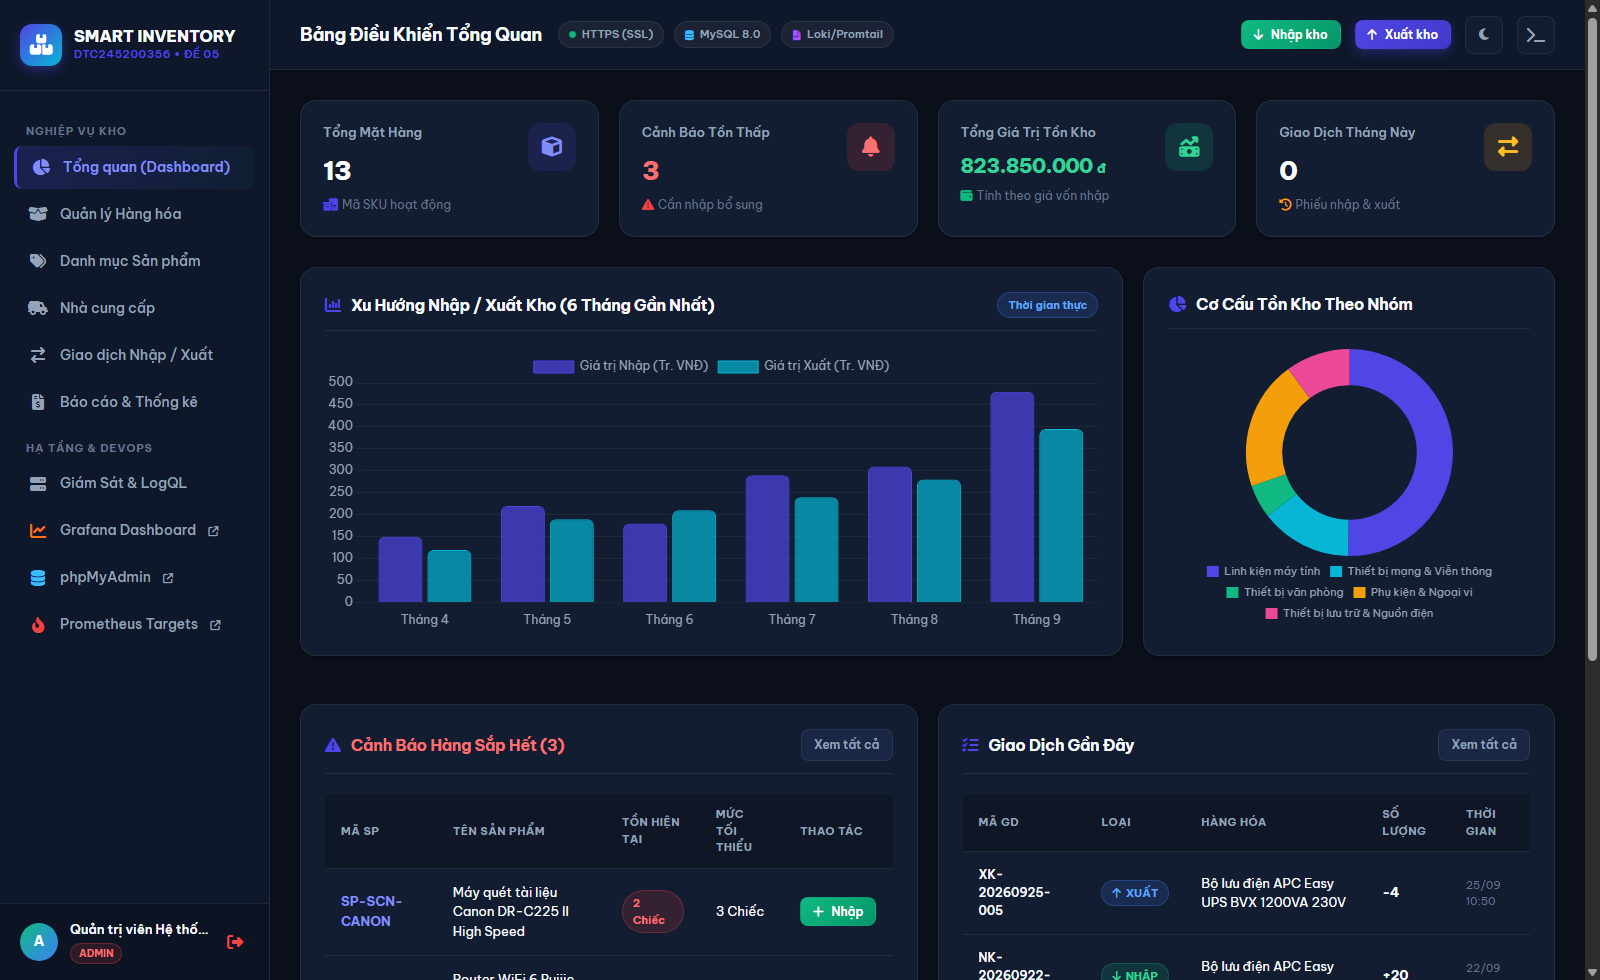
\includegraphics[width=0.98\textwidth,height=0.65\textheight,keepaspectratio]{02_tong_quan_dashboard.png}}
        \end{column}

        \begin{column}{0.44\textwidth}
            \begin{block}{Chỉ Số KPI Thời Gian Thực}
                \begin{itemize}
                    \item \textbf{13 Mặt hàng (SKU):} Hoạt động ổn định.
                    \item \textbf{03 Cảnh báo tồn thấp:} Tồn kho $\le$ \texttt{min\_stock}.
                    \item \textbf{823.850.000 VNĐ:} Tổng vốn định giá kho.
                    \item \textbf{Biểu đồ trực quan:} Xu hướng nhập/xuất 6 tháng \& cơ cấu vốn nhóm hàng.
                \end{itemize}
            \end{block}
            \begin{exampleblock}{Trải Nghiệm Người Dùng}
                Dark Theme hiện đại, font Be Vietnam Pro, bố cục kính mờ Glassmorphism.
            \end{exampleblock}
        \end{column}
    \end{columns}
\end{frame}

% ------------------------------------------------------------------------------
% FRAME 7: NGHIỆP VỤ HÀNG HÓA & IN PHIẾU KHO
% ------------------------------------------------------------------------------
\begin{frame}{6. Phân Hệ Quản Lý Hàng Hóa \& In Phiếu Kho Chuẩn Hóa}
    \begin{columns}[c]
        \begin{column}{0.5\textwidth}
            \centering
            \fbox{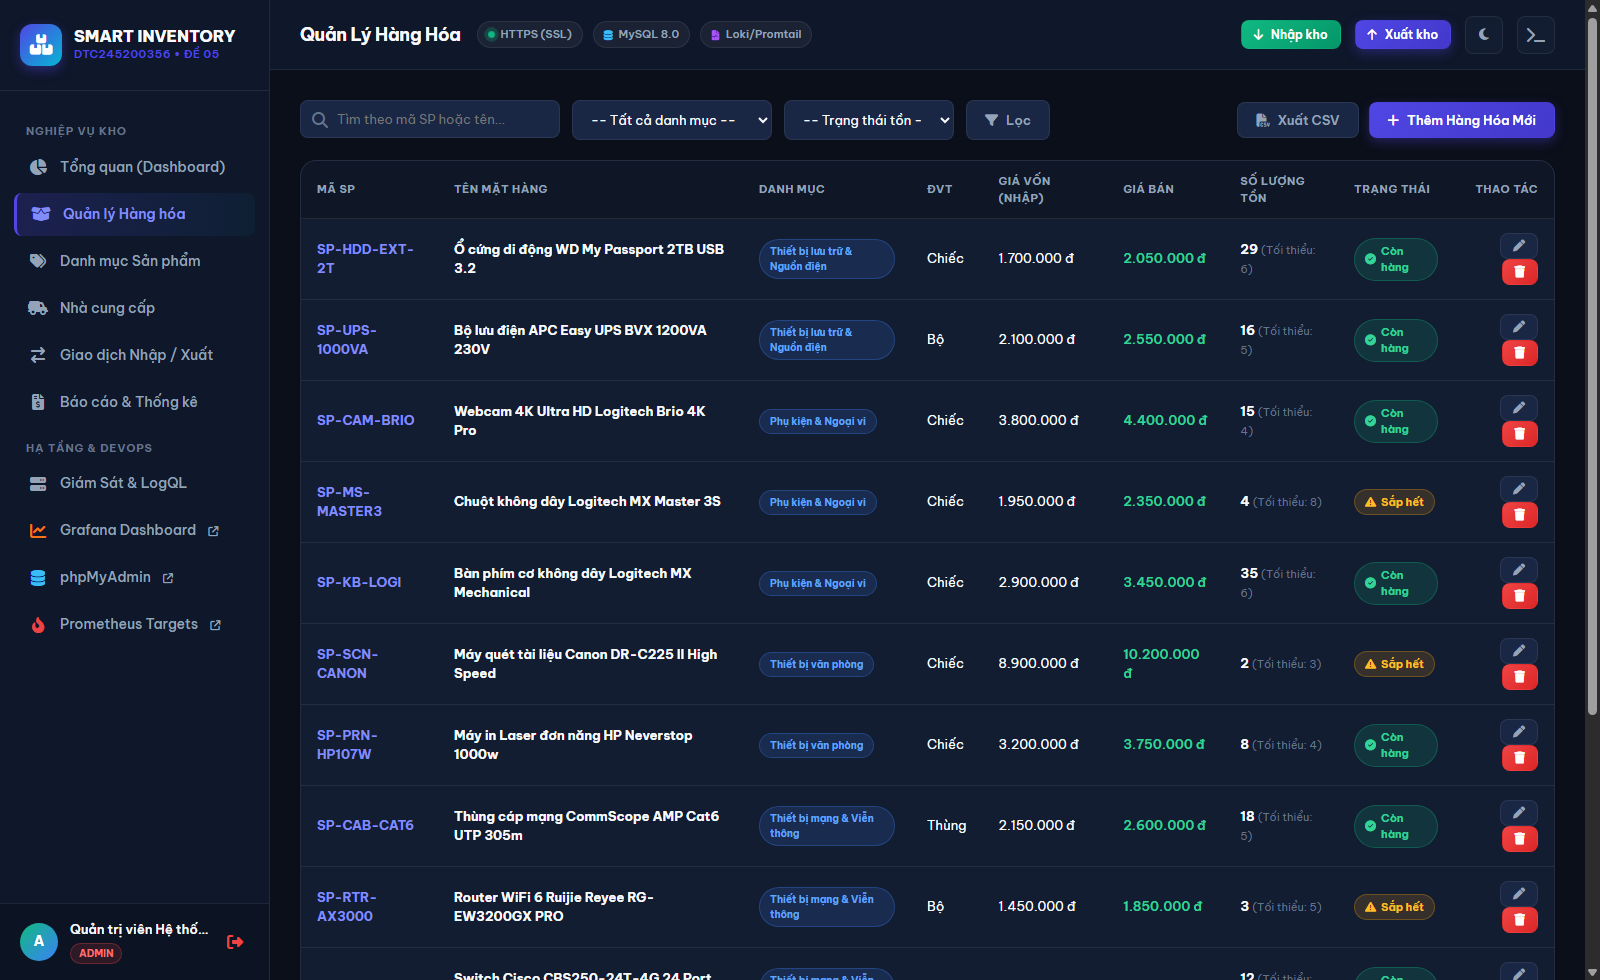
\includegraphics[width=0.96\textwidth,height=0.62\textheight,keepaspectratio]{03_quan_ly_hang_hoa.png}}\\[4pt]
            \footnotesize \textbf{Hình:} Quản lý danh mục sản phẩm, tìm kiếm \& Xuất CSV
        \end{column}

        \begin{column}{0.5\textwidth}
            \centering
            \fbox{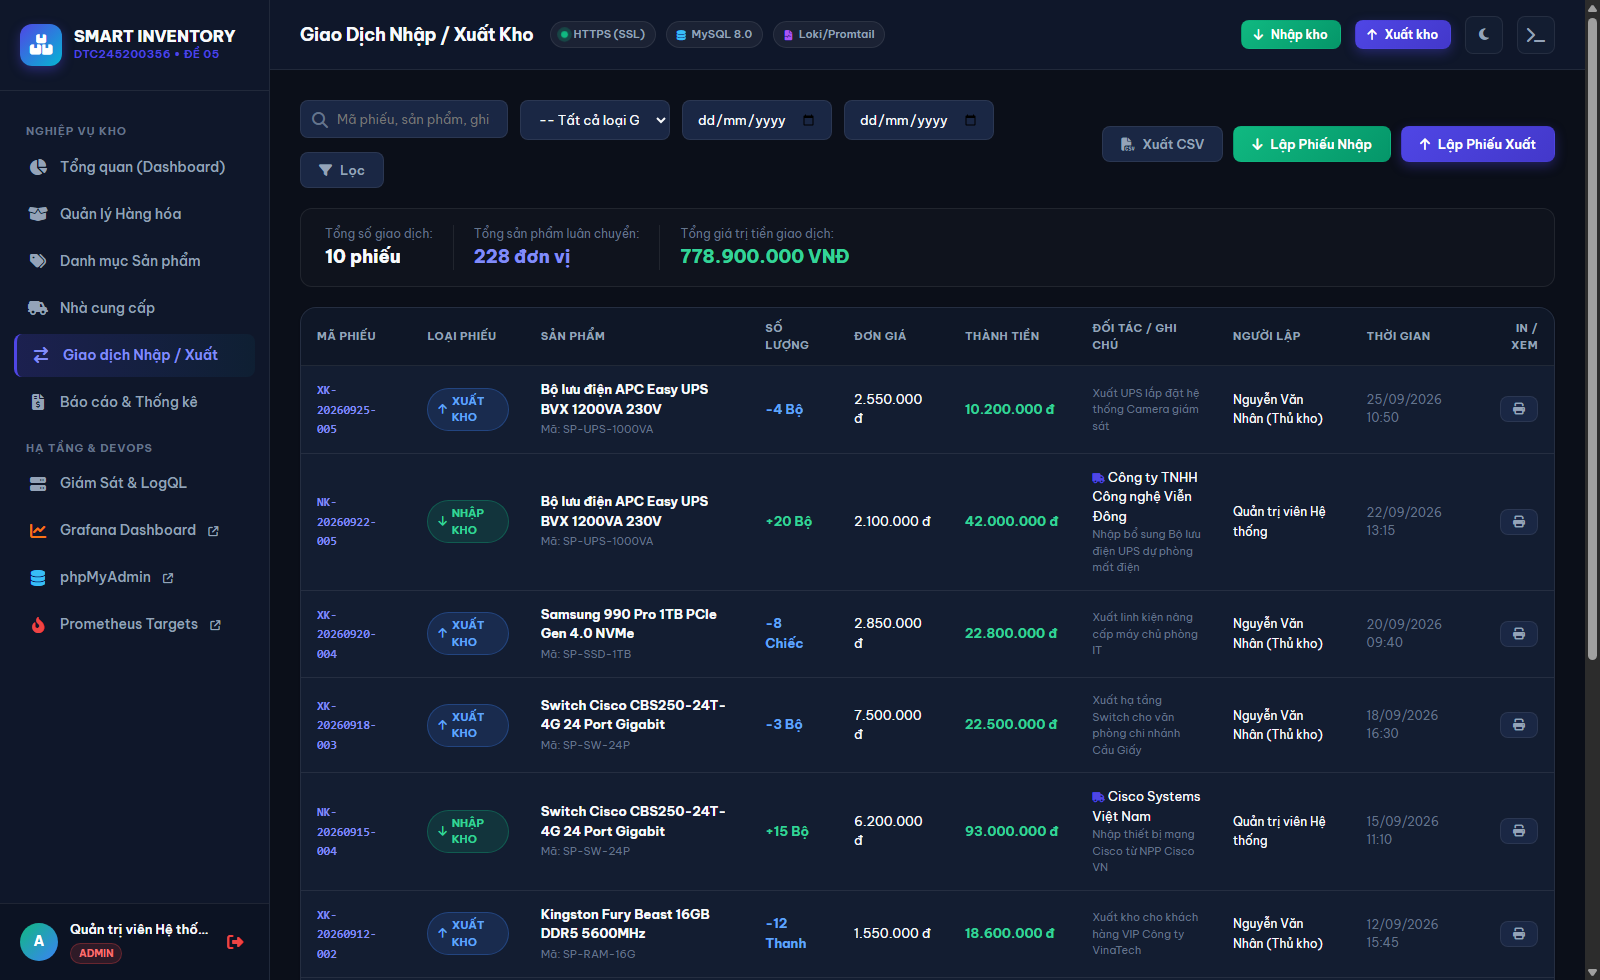
\includegraphics[width=0.96\textwidth,height=0.62\textheight,keepaspectratio]{06_giao_dich_nhap_xuat.png}}\\[4pt]
            \footnotesize \textbf{Hình:} Lịch sử Nhập/Xuất (\texttt{NK}/\texttt{XK}) \& In phiếu kho
        \end{column}
    \end{columns}
\end{frame}

% ------------------------------------------------------------------------------
% FRAME 8: NGINX GATEWAY & SSL (COMMIT 1)
% ------------------------------------------------------------------------------
\begin{frame}[fragile]{7. Nginx Gateway, Mã Hóa SSL \& 5 Security Headers (Commit 1)}
    \begin{columns}[T]
        \begin{column}{0.48\textwidth}
            \begin{block}{Cổng Gateway Bảo Mật}
                \begin{itemize}
                    \item \textbf{Chuyển hướng bắt buộc:} HTTP port 80 sang HTTPS port 443 (\texttt{301 Moved Permanently}).
                    \item \textbf{Chứng chỉ số X.509:} Khóa RSA 2048-bit tự ký có hiệu lực 365 ngày.
                    \item \textbf{Định tuyến URI:} Chuyển tiếp tải vào nội bộ an toàn.
                \end{itemize}
            \end{block}
        \end{column}

        \begin{column}{0.5\textwidth}
            \begin{exampleblock}{5 Tiêu Chuẩn Security Headers}
\begin{lstlisting}
add_header X-Frame-Options "SAMEORIGIN" always;
add_header X-Content-Type-Options "nosniff" always;
add_header X-XSS-Protection "1; mode=block" always;
add_header Referrer-Policy "no-referrer-when-downgrade" always;
add_header Content-Security-Policy 
  "default-src 'self' https: data: 'unsafe-inline' 'unsafe-eval';" always;
\end{lstlisting}
            \end{exampleblock}
        \end{column}
    \end{columns}
\end{frame}

% ------------------------------------------------------------------------------
% FRAME 9: PROMETHEUS METRICS (COMMIT 2)
% ------------------------------------------------------------------------------
\begin{frame}{8. Giám Sát Thời Gian Thực Với Prometheus (Commit 2)}
    \begin{columns}[c]
        \begin{column}{0.54\textwidth}
            \centering
            \fbox{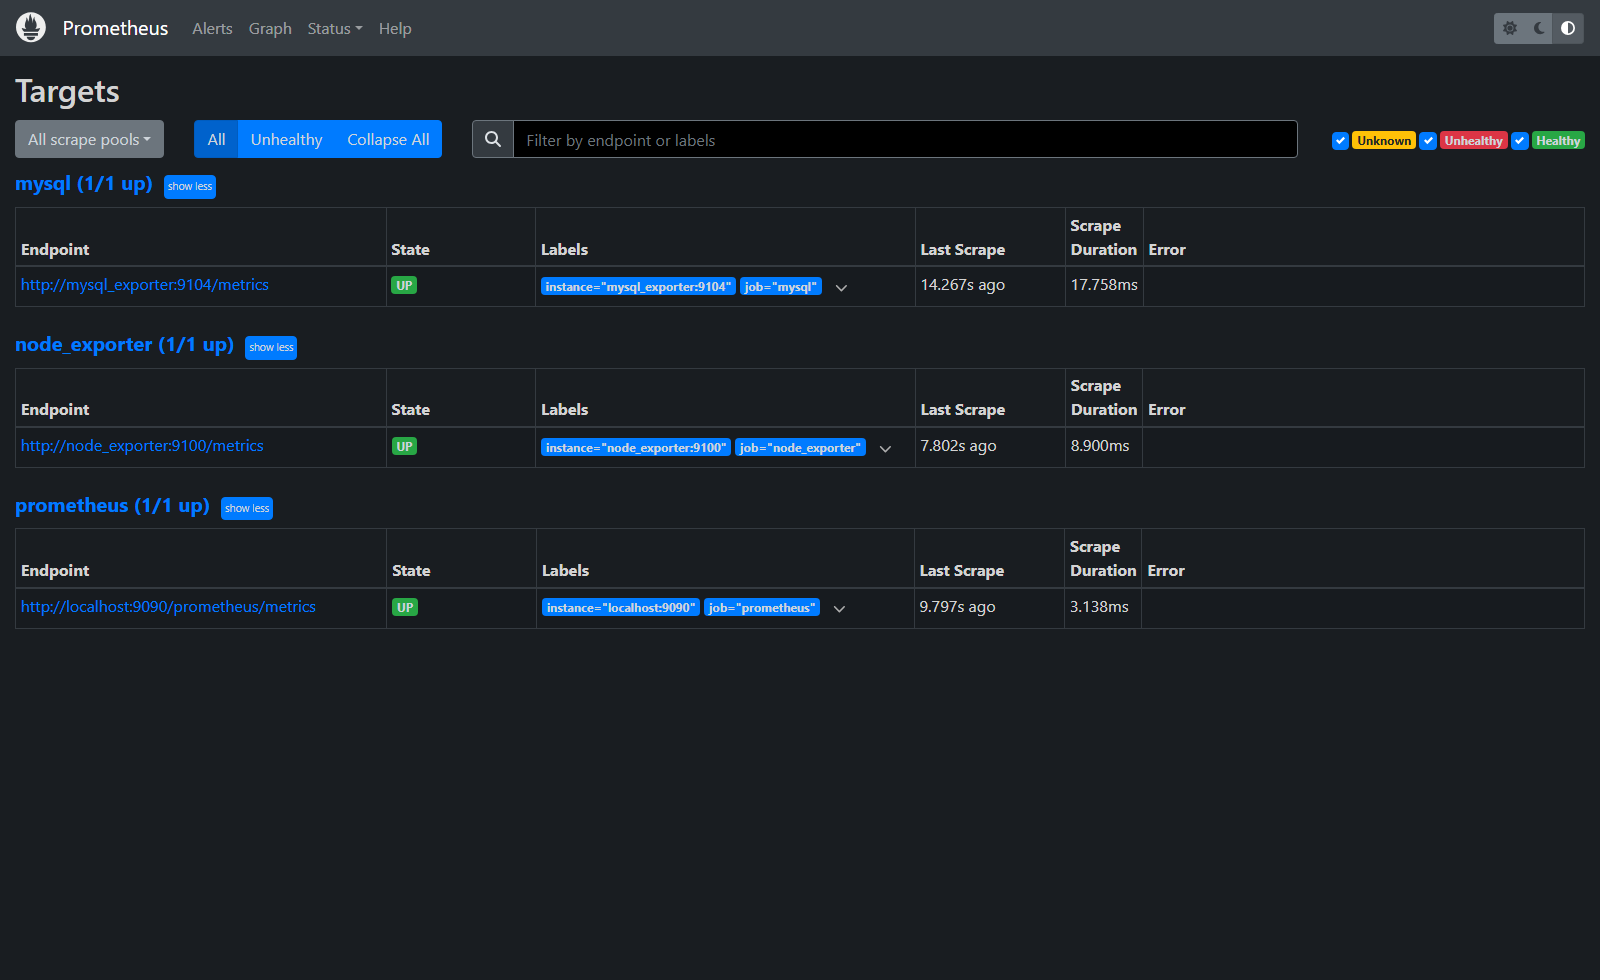
\includegraphics[width=0.98\textwidth,height=0.65\textheight,keepaspectratio]{11_prometheus_targets.png}}
        \end{column}

        \begin{column}{0.44\textwidth}
            \begin{block}{Prometheus Pull Model}
                \begin{itemize}
                    \item Kéo chỉ số định kỳ mỗi \textbf{15 giây} (\texttt{scrape\_interval: 15s}).
                    \item \textbf{100\% Targets đạt trạng thái UP:}
                        \begin{itemize}
                            \item \texttt{mysql\_exporter:9104}: QPS, Connections, Buffer Pool.
                            \item \texttt{node\_exporter:9100}: CPU, RAM, Disk, Network.
                            \item \texttt{prometheus:9090}: Self-monitoring.
                        \end{itemize}
                \end{itemize}
            \end{block}
        \end{column}
    \end{columns}
\end{frame}

% ------------------------------------------------------------------------------
% FRAME 10: GRAFANA PROVISIONING
% ------------------------------------------------------------------------------
\begin{frame}{9. Grafana Dashboard Tự Động Nạp Cấu Hình (Provisioning)}
    \begin{columns}[c]
        \begin{column}{0.54\textwidth}
            \centering
            \fbox{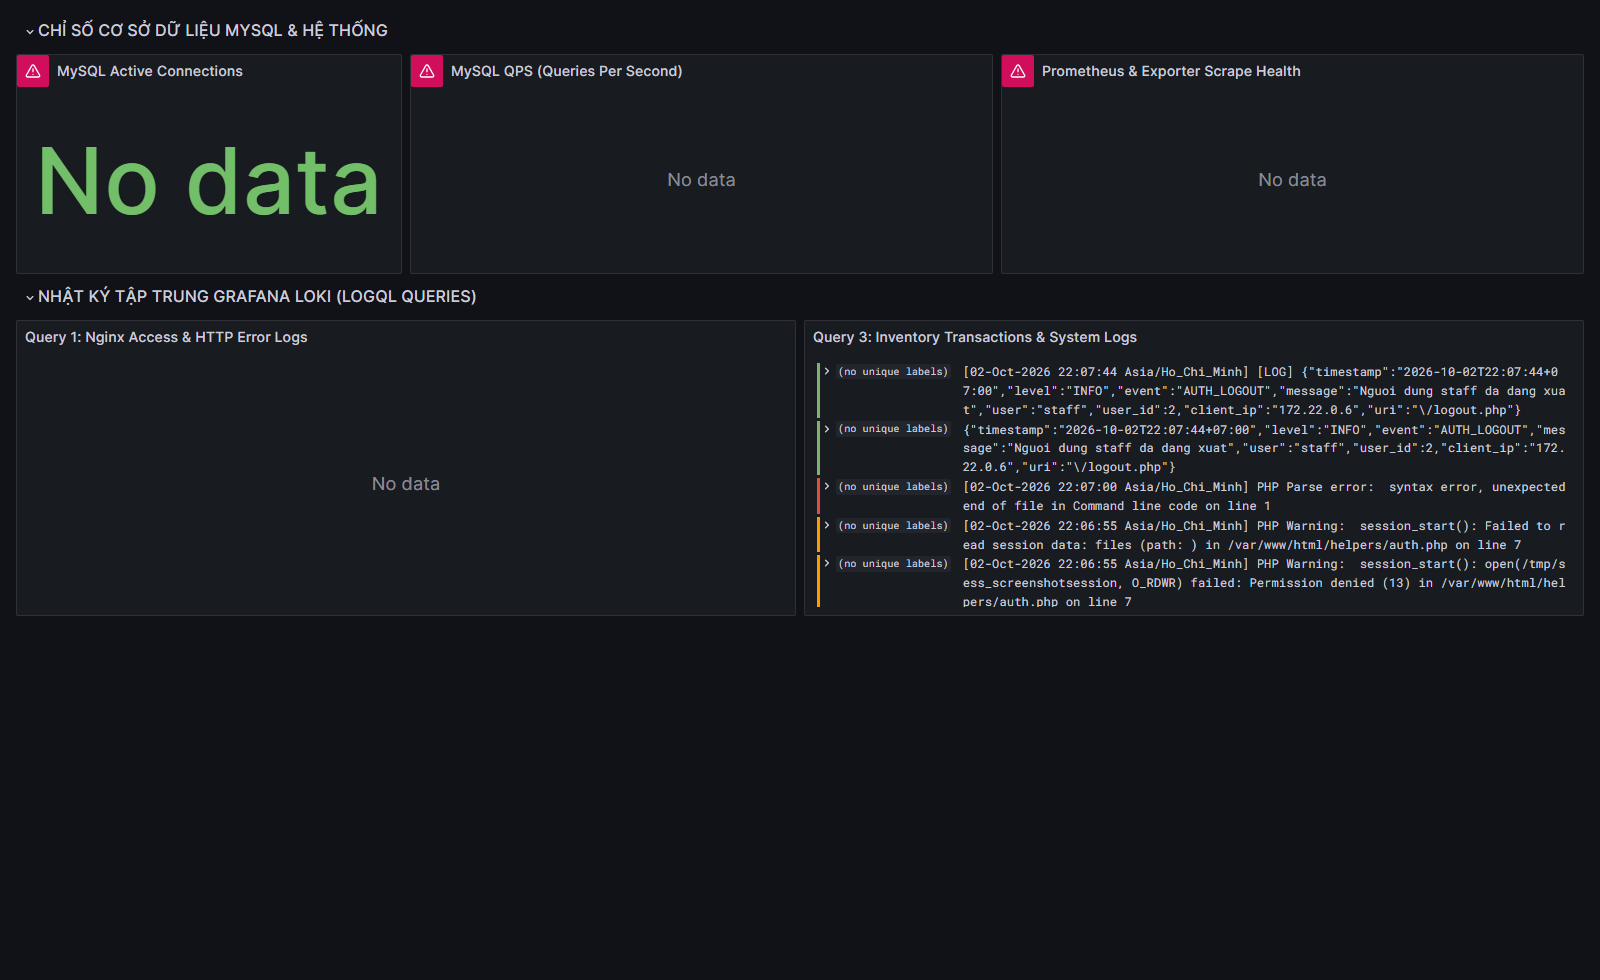
\includegraphics[width=0.98\textwidth,height=0.65\textheight,keepaspectratio]{09_grafana_dashboard.png}}
        \end{column}

        \begin{column}{0.44\textwidth}
            \begin{block}{Cơ Chế Auto-Provisioning}
                \begin{itemize}
                    \item Nạp tự động DataSource Prometheus \& Loki qua tệp cấu hình YAML.
                    \item Tự động khởi tạo Dashboard giám sát không cần thao tác tay.
                \end{itemize}
            \end{block}
            \begin{exampleblock}{Panel Đo Lường Trọng Điểm}
                \begin{itemize}
                    \item MySQL Active Connections.
                    \item Tần suất truy vấn QPS (\texttt{rate}).
                    \item Uptime sức khỏe các dịch vụ.
                    \item Dòng log thời gian thực từ Loki.
                \end{itemize}
            \end{exampleblock}
        \end{column}
    \end{columns}
\end{frame}

% ------------------------------------------------------------------------------
% FRAME 11: LOKI & PROMTAIL LOGGING (COMMIT 3)
% ------------------------------------------------------------------------------
\begin{frame}{10. Quản Lý Nhật Ký Tập Trung Với Loki \& Promtail (Commit 3)}
    \begin{columns}[T]
        \begin{column}{0.48\textwidth}
            \begin{block}{Kiến Trúc Thu Thập Log}
                \begin{enumerate}
                    \item \textbf{Phát sinh log:} Nginx ghi access/error log; Web App ghi JSON log.
                    \item \textbf{Promtail thu gom:} Gắn nhãn metadata (\texttt{job="nginx"}, \texttt{job="app"}) và đẩy về Loki qua HTTP.
                    \item \textbf{Loki lưu trữ:} Đánh index theo labels, nén dữ liệu dung lượng siêu nhỏ.
                \end{enumerate}
            \end{block}
        \end{column}

        \begin{column}{0.48\textwidth}
            \begin{exampleblock}{So Sánh Loki vs ELK Stack}
                \begin{itemize}
                    \item \textbf{Tài nguyên:} Loki tiêu thụ ít RAM hơn Elasticsearch gấp 10 lần.
                    \item \textbf{Đánh chỉ mục:} Chỉ đánh index metadata thay vì toàn văn tốn kém.
                    \item \textbf{Tích hợp:} Native 100\% với giao diện Grafana có sẵn.
                    \item \textbf{Truy vấn:} Cú pháp LogQL trực quan, tương đồng PromQL.
                \end{itemize}
            \end{exampleblock}
        \end{column}
    \end{columns}
\end{frame}

% ------------------------------------------------------------------------------
% FRAME 12: 3 LOGQL QUERIES & SANDBOX
% ------------------------------------------------------------------------------
\begin{frame}[fragile]{11. Phân Tích Sự Cố Với 3 Câu Truy Vấn LogQL Chuyên Sâu}
    \begin{columns}[T]
        \begin{column}{0.5\textwidth}
            \begin{block}{3 Câu Truy Vấn LogQL Cốt Lõi}
\textbf{1. Lọc lỗi HTTP 4xx/5xx Nginx Gateway:}
\begin{lstlisting}
{job="nginx"} |= "status=" |~ "status=[45][0-9][0-9]"
\end{lstlisting}
\textbf{2. Thống kê request theo IP (Phát hiện DoS):}
\begin{lstlisting}
sum by (client_ip) (count_over_time({job="nginx"} [5m]))
\end{lstlisting}
\textbf{3. Truy vết lỗi giao dịch kho hàng App:}
\begin{lstlisting}
{job="app"} |= "inventory_transactions" |= "ERROR"
\end{lstlisting}
            \end{block}
        \end{column}

        \begin{column}{0.48\textwidth}
            \centering
            \fbox{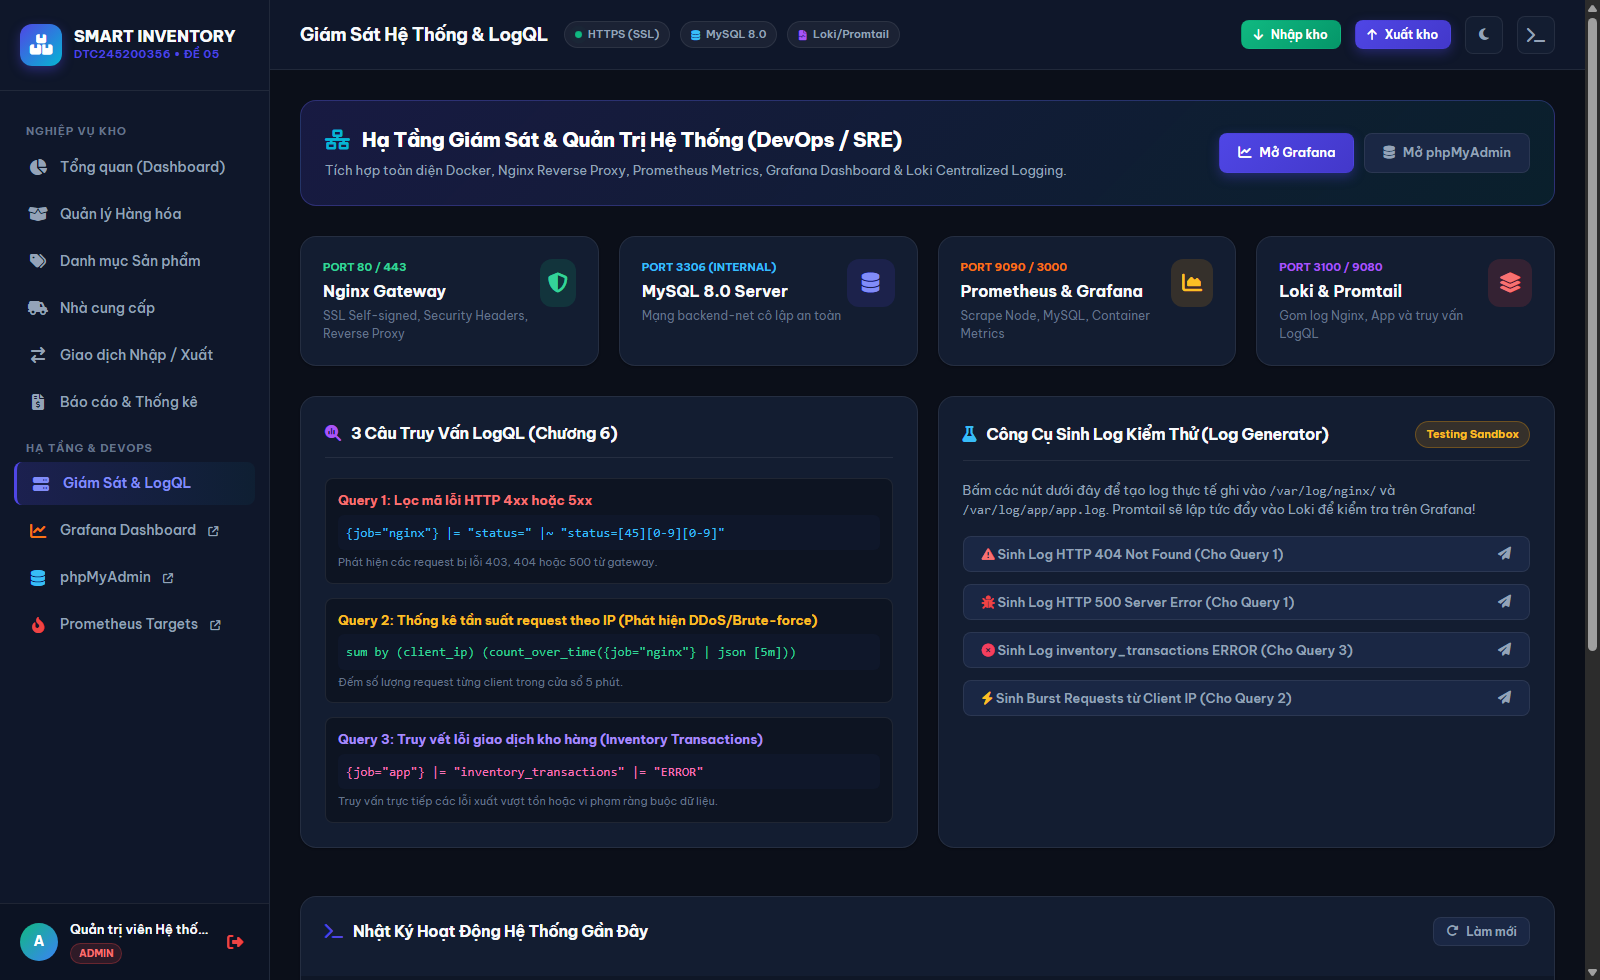
\includegraphics[width=0.98\textwidth,height=0.62\textheight,keepaspectratio]{08_trung_tam_giam_sat_logql.png}}\\[4pt]
            \footnotesize \textbf{Hình:} Trung tâm DevOps \& Sandbox sinh log giả lập để kiểm thử trực tiếp
        \end{column}
    \end{columns}
\end{frame}

% ------------------------------------------------------------------------------
% FRAME 13: GIA CỐ BẢO MẬT (HARDENING)
% ------------------------------------------------------------------------------
\begin{frame}{12. Gia Cố Bảo Mật Hệ Thống Theo Chuẩn CIS Docker Benchmark}
    \begin{columns}[T]
        \begin{column}{0.48\textwidth}
            \begin{block}{1. Non-Root User Container}
                Chạy ứng dụng bằng tài khoản hạn chế \texttt{appuser (UID 1001)}. Triệt tiêu rủi ro chiếm đoạt quyền root máy chủ host khi container bị khai thác (\textit{Container Breakout}).
            \end{block}
            \begin{block}{2. Phân Vùng Mạng Cô Lập}
                Tách 3 mạng Docker bridge: \texttt{frontend-net}, \texttt{backend-net}, \texttt{monitoring-net}. Cơ sở dữ liệu MySQL \textbf{khóa cổng 3306}, không lộ ra Internet.
            \end{block}
        \end{column}

        \begin{column}{0.48\textwidth}
            \begin{exampleblock}{3. Quản Lý Bí Mật An Toàn}
                Tách biệt file \texttt{.env}, đưa vào \texttt{.gitignore} ngăn ngừa rò rỉ mã nguồn lên GitHub; cung cấp mẫu \texttt{.env.example} chuẩn.
            \end{exampleblock}
            \begin{exampleblock}{4. Giới Hạn Trần Tài Nguyên}
                Thiết lập CPU và RAM limit cho từng container (MySQL: 1.0 CPU, 1GB RAM; Web: 0.75 CPU, 512MB RAM), phòng chống tấn công cạn kiệt tài nguyên máy chủ.
            \end{exampleblock}
        \end{column}
    \end{columns}
\end{frame}

% ------------------------------------------------------------------------------
% FRAME 14: KIỂM THỬ THỰC NGHIỆM (10/10 PASS)
% ------------------------------------------------------------------------------
\begin{frame}{13. Ma Trận Đánh Giá \& Kiểm Thử Thực Nghiệm (10/10 PASS)}
    \begin{center}
        \scriptsize
        \begin{tabular}{c l p{0.45\textwidth} c}
            \toprule
            \textbf{Mã} & \textbf{Hạng Mục} & \textbf{Kịch Bản Thực Nghiệm \& Kết Quả} & \textbf{Đánh Giá} \\
            \midrule
            TC-01 & Xác thực & Phân quyền RBAC, mật khẩu BCRYPT, bảo vệ cookie phiên & \textbf{PASS} \\
            TC-02 & Nhập kho & Tăng tồn chính xác (+15), tự động sinh mã phiếu \texttt{NK-xxxx} & \textbf{PASS} \\
            TC-03 & Xuất kho & Khấu trừ tồn kho an toàn, lưu lịch sử thủ kho \& đối tác & \textbf{PASS} \\
            TC-04 & Chặn xuất âm & Từ chối xuất vượt tồn kho, rollback DB, ghi log ERROR & \textbf{PASS} \\
            TC-05 & Cảnh báo tồn & Phát hiện 3 mặt hàng dưới ngưỡng \texttt{min\_stock}, gắn badge cảnh báo & \textbf{PASS} \\
            TC-06 & HTTPS 301 & Chuyển hướng 100\% lưu lượng HTTP port 80 sang HTTPS port 443 & \textbf{PASS} \\
            TC-07 & Security Headers & Đạt đủ 5/5 tiêu chuẩn an ninh: CSP, X-Frame, nosniff, X-XSS & \textbf{PASS} \\
            TC-08 & Cô lập MySQL & Port 3306 bị từ chối từ Host, chỉ kết nối nội bộ trong backend-net & \textbf{PASS} \\
            TC-09 & Scrape Target & 100\% Exporters (\texttt{mysql}, \texttt{node}, \texttt{prometheus}) đạt trạng thái UP & \textbf{PASS} \\
            TC-10 & LogQL Queries & Promtail gom log, thực thi lọc khớp 100\% lỗi 4xx/5xx \& nghiệp vụ & \textbf{PASS} \\
            \bottomrule
        \end{tabular}
    \end{center}
    \begin{exampleblock}{Kết Luận}
        Tỷ lệ hoàn thành: \textbf{100\% (10/10 ca kiểm thử PASS)}. Hệ thống đạt độ tin cậy và sẵn sàng vận hành.
    \end{exampleblock}
\end{frame}

% ------------------------------------------------------------------------------
% FRAME 15: KẾT LUẬN & HƯỚNG PHÁT TRIỂN
% ------------------------------------------------------------------------------
\begin{frame}{14. Kết Luận \& Lộ Trình Nâng Cấp Tương Lai}
    \begin{columns}[T]
        \begin{column}{0.48\textwidth}
            \begin{block}{Thành Quả Đạt Được}
                \begin{itemize}
                    \item Hoàn thành xuất sắc 100\% yêu cầu Đề tài số 05.
                    \item Website quản lý kho hoàn chỉnh nghiệp vụ, Dark UI cao cấp, in phiếu kho, xuất CSV.
                    \item Cụm 10 container vi dịch vụ điều phối an toàn qua Docker Compose.
                    \item Cổng Nginx Gateway bảo mật SSL \& Security Headers.
                    \item Giám sát thời gian thực Prometheus, Grafana Auto-provisioning \& Gom log Loki LogQL.
                \end{itemize}
            \end{block}
        \end{column}

        \begin{column}{0.48\textwidth}
            \begin{exampleblock}{Lộ Trình Nâng Cấp Kỹ Thuật}
                \begin{itemize}
                    \item \textbf{CI/CD GitHub Actions:} Tự động kiểm thử, build image và đẩy lên Docker Hub.
                    \item \textbf{Let's Encrypt SSL:} Cấp phát tự động chứng chỉ số công khai có độ tin cậy toàn cầu bằng Certbot.
                    \item \textbf{Kubernetes (K8s/K3s):} Nâng cấp lên cụm K8s với tính năng tự phục hồi (Self-healing) và tự động mở rộng theo tải (HPA).
                \end{itemize}
            \end{exampleblock}
        \end{column}
    \end{columns}
\end{frame}

% ------------------------------------------------------------------------------
% FRAME 16: HỎI ĐÁP & LIVE DEMO
% ------------------------------------------------------------------------------
\begin{frame}{15. Phiên Hỏi Đáp (Q\&A) \& Trình Diễn Hệ Thống (Live Demo)}
    \begin{center}
        \Huge \textbf{\textcolor{techaccent}{XIN TRÂN TRỌNG CẢM ƠN}}\\[6pt]
        \Large \textbf{THẦY CÔ VÀ HỘI ĐỒNG ĐÃ LẮNG NGHE!}\\[14pt]
        
        \normalsize
        \begin{tabular}{rl}
            \textbf{Repository GitHub:} & \texttt{cuongcoder123/DTC245200356-QLKH} \\
            \textbf{Email liên hệ:} & \texttt{DTC245200356@ictu.edu.vn} \\
            \textbf{Cổng truy cập Demo:} & \texttt{https://localhost/} (Web App) \\
            & \texttt{https://localhost/grafana/} (Grafana Dashboard) \\
            & \texttt{https://localhost/prometheus/} (Scrape Targets)
        \end{tabular}
        
        \vspace{12pt}
        \begin{exampleblock}{\centering SẴN SÀNG CHO PHẦN TRÌNH DIỄN THỰC TẾ (LIVE DEMO)}
            Kính mời Thầy Cô và Hội đồng đặt câu hỏi phản biện và đánh giá đề tài!
        \end{exampleblock}
    \end{center}
\end{frame}

\end{document}
